%-----------------------------------------------------------
%   Capítulo 6 - Implementação
%-----------------------------------------------------------
\chapter{Implementação}

Neste capítulo vai ser descrita a implementação do sistema do ponto de vista do \textit{hardware} e \textit{software}.


\section{\textit{Hardware}}

Em relação ao \textit{hardware}, as conexões estão representadas na figura \ref{hard}.
\\O circuito é composto por 8 LDRs, conectados a 8 resistências, que são alimentados por 3.3 volts. Cada um dos LDR está conectado a um pino ADC do STM32, o mesmo também tem o RX conectado ao RX do \textit{transciever} e o TX da mesma forma. O H (\textit{higth}) e o L (\texit{low}) estão conectados no barramento do \textit{master}.

\begin{figure}[!htb]
\centering
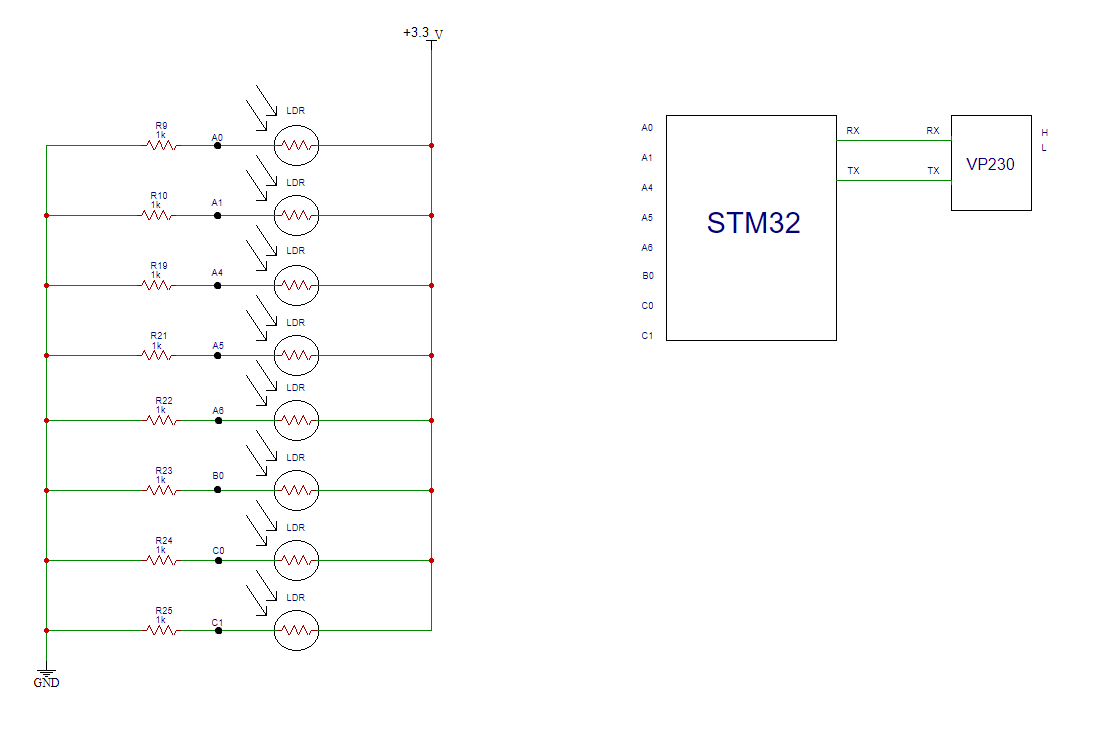
\includegraphics[scale=0.55]{Figuras/circuito.PNG}
\caption{Conexões com os sensores}
\label{hard}
\end{figure}

\newpage

\section{\textit{Software}}

O código desenvolvido para este projeto pode ser dividido em duas partes: a leitura dos sensores que comunicam por ADC e a transferência de dados pelo protocolo de comunicação CAN.
\\No protocolo CAN as variáveis que mais têm implicações na comunicação, é o ID e os quatro primeiros \texit{bytes} de dados.

\subsection{Leitura dos valores ADC dos LDR}

A leitura dos LDR é realizada através da comunicação ADC com
\textit{direct memory access} (DMA).

Na figura \ref{adc} está representada a função para realizar a leitura dos LDR.

\begin{figure}[!htb]
\centering
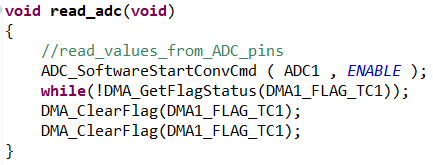
\includegraphics[scale=1]{Figuras/adc.PNG}
\caption{Função para leitura dos sensores}
\label{adc}
\end{figure}

\newpage

\subsection{Envio dos valores para o \textit{master}}

Para comunicar com o \textit{master} é utilizado o protocolo CAN, na figura \ref{can}, está representada a função para comunicação CAN.
\\Na função inicialmente é verificado se existe alguma tentativa de comunicação por parte \textit{master}, caso isso se confirme, os dados são obtidos e verifica-se se a informação é direccionada ao \textit{slave} pelo qual estamos responsáveis, se for verdade, são preenchidos os dados com a mensagem a ser enviada para o \textit{master} e por fim é realizada a transmissão.   

\newpage
\begin{figure}[!htb]
\centering
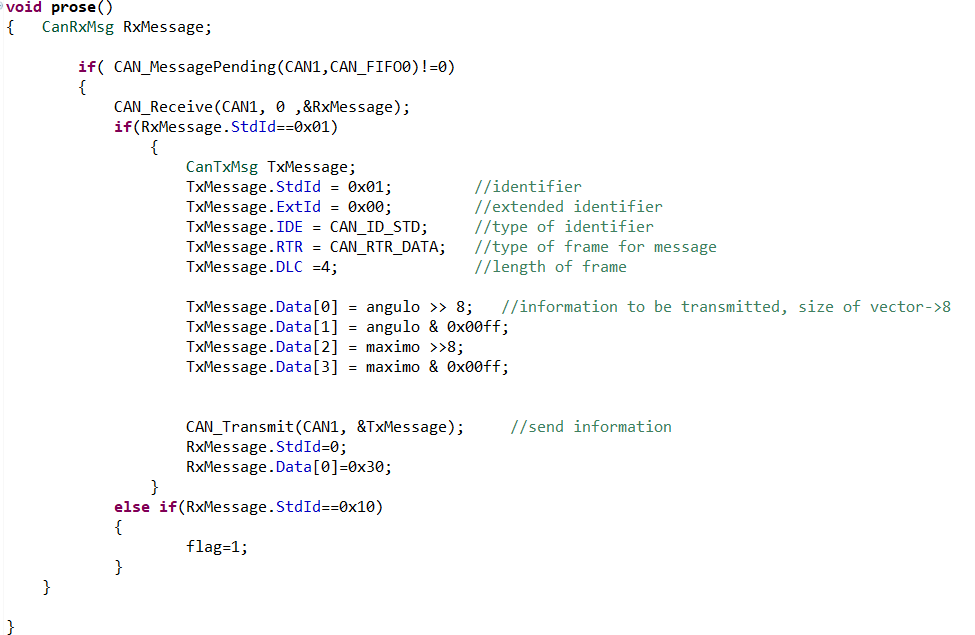
\includegraphics[scale=0.7]{Figuras/can.PNG}
\caption{Função para envio dos dados para o \textit{master}}
\label{can}
\end{figure}

Para converter os valores de resistivos do LDR para Lux é utilizada a formula 3.1, a fórmula foi obtida a partir do \texit{datasheet} do LDR.

\begin{equation} 
    {Lux=4000000*R^{-1.303}}
\end{equation}


\\Na figura \ref{roll}, é demonstrado como é feito a conversão de Lux para roll, são obtidos os dois maiores valores em Lux e a sua posições no anel, e a partir da diferença dos dois é calculado o valor do roll, a equação 3.2 demostra essa relação.

\begin{equation} 
    {ang=(pos*45*MaxLux+pos2*45*2MaxLux)/(MaxLux+2MaxLux)}
\end{equation}

\newpage
\begin{figure}[!htb]
\centering
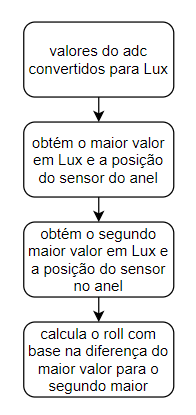
\includegraphics[scale=0.7]{Figuras/roll.PNG}
\caption{Calculo do roll}
\label{roll}
\end{figure}


